\documentclass[a4paper,13pt]{article}

%%%%%%%%%%%%%%%%%%%%%%%%%%%%%%%%%%%%%%%%%%%%%%%%%%%%%%%%%%%%

% Global structure parameters
\usepackage{fullpage}%

\usepackage[francais]{babel}%

\usepackage[utf8]{inputenc}%
\usepackage[T1]{fontenc}%

\usepackage{mathpazo}%

% Macro packages
\usepackage{url}%
\usepackage{graphicx}%
\usepackage{minted}%
\usemintedstyle{borland}%

% for algorithm
\usepackage[french, onelanguage]{algorithm2e}
\usepackage{algorithmic}
% for tree
\usepackage{tikz}
\usepackage{amsmath}

%for floaw chart
\usetikzlibrary{arrows.meta}
\tikzset{%
  >={Latex[width=2mm,length=2mm]},
  % Specifications for style of nodes:
            base/.style = {rectangle, rounded corners, draw=black,
                           minimum width=4cm, minimum height=1cm,
                           text centered, font=\sffamily},
  mainFile/.style = {base, fill=blue!30},
       subFile/.style = {base, fill=red!30},
    module/.style = {base, fill=green!30},
        % process/.style = {base, minimum width=2.5cm, fill=orange!15,font=\ttfamily},
}

\usepackage{ragged2e}

\RestyleAlgo{boxruled}
\SetAlCapHSkip{0.5em}
\IncMargin{1em}

% Fine tuning
\setlength{\parskip}{0.2\baselineskip plus 0.2\baselineskip}%

%%%%%%%%%%%%%%%%%%%%%%%%%%%%%%%%%%%%%%%%%%%%%%%%%%%%%%%%%%%%

\begin{document}

\title{Rapport Projet 0: Tours d'Hanoï et Pavage de Penrose}

\author{Bailluet Nicolas, Rémi Piau}

%\date{11 septembre 2018}

\maketitle

\begin{abstract}
  Ceci est un résumé.
\end{abstract}

%%%%%%%%%%%%%%%%%%%%%%%%%%%%%%%%%%%%%%%%%%%%%%%%%%%%%%%%%

\section{Les tours de Hanoï}

Nous traitons dans cette partie le problème des tours de Hanoï à $n$ disques et 3 piquets. Nous exposons dans un premier temps une solution récursive classique, son étude nous mène par la suite à contruire une solution itérative.

\subsection{Solution initiale - Un algortithme récursif}

La résolution du problème est basée sur le fait que pour déplacer un disque d'un piquet à un autre, il est nécessaire de déplacer tous les disques présents au dessus sur un piquet intermédiaire. Ainsi, pour résoudre le problème à $n$ disques on effectue les actions suivantes (voir l'algorithme~\ref{alg:hanoirec}):
\begin{itemize}
  \item résoudre le problème pour $n-1$ disques qui sont déplacés vers un piquet intermédiaire;
  \item déplacer le $n$-ieme disque vers le piquet d'arrivée;
  \item résoudre le problème pour $n-1$ disques qui sont déplacés du piquet intermédiaire vers le piquet d'arrivée.
\end{itemize}

\bigskip
Une solution simple et optimale en nombre de coups joués. En effet, notons $C(n)$ le nombre de coups nécessaire, alors:\newline
\begin{center}
$
C(n) =
    \begin{cases}
      1 & \mbox{si $n$ = 1}\\
      2C(n-1)+1 & \mbox{sinon}
    \end{cases}
$
$
\Leftrightarrow \boxed{C(n) = 2^{n}-1}
$
\end{center}

\subsection{Étude de la résolution récursive}

Afin de construire l'algorithme itératif, il est tout d'abord nécessaire de montrer certaines propriétés relative à la résolution récursive décrite précedemment.

\subsubsection{Représentation arborescente}

Nous utiliserons par la suite une représentation arborescente des appels récursifs (et des tours de jeu). Pour cela nous indiçons les disques de 1 (le plus petit) à $n$ (le plus grand).
L'arbre suit le schéma suivant :
\begin{itemize}
  \item on place à la racine le noeud étiqueté $n$ correspondant au premier appel récursif;
  \item tout noeud a pour fils gauche l'arbre pour $n⁻1$ disques, ce qui représente les pré-requis pour pouvoir déplacer le disque d'indice $n$;
  \item tout noeud a pour fild droit l'arbre pour $n-1$ disques, ce qui représente les actions à effectuer après le mouvement du disque d'indice $n$ afin de pouvoir reformer la tour.
\end{itemize}

Un exemple pour $n=4$ se trouve en annexe (voir figure~\ref{fig:arbre4}).
\bigskip

Par construction, l'arbre binaire est complet, son parcours infixe donne l'ordre de jeu des disques et tous les noeuds d'une même génération possèdent la même étiquette. Ainsi en considérant le premier tour de jeu comme le tour d'ordre 0 on en déduit :
\begin{center}
  \emph{Le plus petit disque est joué à tous les tours d'ordre pair.}
\end{center}

\subsubsection{Direction des disques}

Nous pouvons de plus montrer \emph{qu'un même disque est toujours déplacé de la même manière, soit d'un piquet vers la droite, soit d'un piquet vers la gauche}.\par
Soit $k \in \{ 1, ..., n\}$, notons $c_{k}(i)$ le triplet (piquet de départ, piquet intermédiaire, piquet d'arrivée) lors du $i$-ieme mouvement du disque d'indice $k$. Montrons par récurrence descendante sur $k$ que $c_{k}(i+1)$ est une rotation de $c_{k}(i)$ vers la droite:
\begin{itemize}
  \item pour $k=n$, il n'y a qu'un seul mouvement du disque d'indice $k$;
  \item supposons le résultat vrai pour un $k'$ et notons $c_{k}(i) = (a,b,c)$ (pour un $i$ fixé) :
    \begin{itemize}
      \item si $i$ est pair, alors $c_{k'-1}(\frac{i}{2}) = (a,c,b)$ d'où $c_{k'}(i+1) = (c,a,b)$ (voir l'algorithme~\ref{alg:hanoirec});
      \item sinon, alors $c_{k'-1}(\frac{i-1}{2}) = (b,a,c)$ puis par hypothèse de récurrence $c_{k'-1}(\frac{i+1}{2}) = (c,b,a)$ et donc $c_{k'}(i+1) = (c,a,b)$.
    \end{itemize}
\end{itemize}

D'où le résultat.

\subsubsection{Étude du tour de jeu d'ordre $k$}

Nous pouvons ensuite déterminer l'indice du disque joué au tour d'ordre $k$. On remarque pour cela que la parcours infixe de l'arbre pour $n$ disques auquel on retire tous les 1 donne le parcours de l'arbre pour $n-1$ disques (le plus petit disque est alors indicé 2), ainsi un noeud interne situé en $k$-ieme position dans le parcours pour $n$ disque est situé en position $\frac{k-1}{2}$ dans le parcours pour $n-1$ disques. De plus on sait que les tours d'ordre pair correspondent au mouvements du plus petit disque. Ainsi pour déterminer l'indice du disque joué on procède comme ceci :
\begin{itemize}
  \item si $k$ est pair, le plus petit disque est joué;
  \item sinon on réitère le procédé avec $\frac{k-1}{2}$, et l'indice du disque joué est le nombre de fois qu'il a été nécessaire de diviser $k$.
\end{itemize}

\bigskip
Autrement dit:
\begin{center}
  \emph{L'indice du disque joué au tour d'ordre $k$ est l'indice du premier bit nul dans l'écriture binaire de $k$.}
\end{center}

\subsection{Solution itérative}

Il est alors possible à partir des propriétés démontrées de construire un algorithme itératif. Pour cela on effectue les mouvements suivants tant que le piquet d'arrivée ne contient pas $n-1$ disques:
\begin{itemize}
  \item déplacer le plus petit disque vers la droite ou la gauche en fonction de la parité de $n$;
  \item faire le seul mouvement qui n'implique pas de déplacer le plus petit disque.
\end{itemize}
Il reste alors à déplacer le plus petit disque vers le piquet d'arrivée (voir l'algorithme~\ref{alg:hanoiiter}).
\bigskip

La terminaison, l'optimalité et la correction sont immédiates par construction, les mouvements sont les mêmes que celui de l'algorithme récursif qui est correct et optimal.

\subsection{Implémentation}

Afin de gérer le contenu de chaque piquet, le type abstrait \emph{Rod} a été implémenté (voir l'interface en annexe figure~\ref{fig:rod}):
\mintinline{ocaml}{type rod =
{ mutable size: int; name: string; mutable discs: int list}}, l'implémentation ressemble à celle d'une pile et ne tient pas compte des règles du jeu, il est donc possible de l'utiliser dans le cas où l'on souhaiterait changer les règles.\par

Afin de mieux visualiser la résolution, nous avons implémenté une animation qui affiche le schéma de résolution. Les disques sont représentés par des rectangles et celui en mouvement est coloré en rouge (voir la figure~\ref{fig:hanoiimg}).

%%%%%%%%%%%%%%%%%%%%%%%%%%%%%%%%%%%%%%%%%%%%%%%%%%%%%%%%%

\section{Pavage de Penrose}

Nous nous intéressons au pavage de penrose sur un exemple avec des triangles isocèles de rapport $\phi$ entre leurs côtés (avec $\phi = \frac{1 + \sqrt{5}}{2}$, le nombre d'or).

\subsection{Solution initiale - Algorithme: un pavage par découpage récursif}
L'algorithme proposé pour le pavage est un découpage récursif d'un triangle de départ en sous triangles (voir l'algorithme~\ref{alg:penrose}). Le découpage diffère en fonction de la nature du triangle obtu ou aïgu (voir figure~\ref{fig:decoupage1}).
En reprenant les notations de la figure~\ref{fig:decoupage1}, on peut écrire les formules de découpage qui reviennent à calculer la position du point $D$ dans le cas obtu et des points $D$ et $E$ dans l'autre cas. On a (avec $O$ l'origine du repère i.e $(0,0)$):
\[ \vec{OD} = \vec{OA} + \frac{\vec{AB}}{\phi}\]
pour le triangle obtu, et
\[ \vec{OD} = \vec{OC} - \frac{\vec{AC}}{\phi}\]

\[ \vec{OE} = \vec{OB} + \frac{\vec{BC}}{\phi}\]
pour le triangle aïgu.
\subsection{Implémentation: un code modulaire}

L'implémentation du pavage à été divisée en plusieurs fichiers (voir figure~\ref{fig:filesrelation} pour les relations entre ces fichiers, une flèche vers un fichier indique que celui-ci est utilisé par celui d'où part la flèche).



\subsubsection{Une interface de programmation pour les triangles: \mintinline{text}{api\_triangle.cma}}
Nous avons réalisé une interface de programmation \mintinline{text}{api_triange.cma}.

Cette interface [\ref{code:apitrianglemli}] expose plusieurs types abstraits:
\begin{itemize}
	\item les types d'angle, aîgus ou obtus \mintinline{ocaml}{type angletype = Obtuse | Acute},
	\item les points représentés par un couple de flottant i.e. \mintinline{ocaml}{type point = (float * float)},
	\item les triangles \mintinline{ocaml}{type triangle = {points:(point array); typ:angletype}}, repésentés par une liste de points et un type d'angle.
\end{itemize}
Ces types sont accessibles et manipulables \emph{uniquement} travers des fonctions exposées par l'interface comme la fonction \mintinline{ocaml}{is_acute : triangle -> bool}. On notera l'implémentation d'opérateurs infixes comme \mintinline{ocaml}{-- : point -> point -> point}(soustraction) ou \mintinline{ocaml}{// : point -> float -> point}(division par un scalaire) qui permettent de manipuler le type point de manière élégante et plus compréhensible.
\begin{itemize}
	\item les type d'angles, aîgus ou obtus \mintinline{ocaml}{type angletype = Obtuse | Acute},
	\item les points représentés par un couple de flottant i.e. \mintinline{ocaml}{type point = (float * float)},
	\item les triangle \mintinline{ocaml}{type triangle = {points:(point array); typ:angletype}}, repésentés par une liste de points et un type d'angle.
\end{itemize}
Ces types ne sont accessibles et manipulables \emph{uniquement} travers des fonctions exposées par l'interface comme la fonction \mintinline{ocaml}{is_acute : triangle -> bool}. On notera l'implémentation d'opérateurs infixe comme \mintinline{ocaml}{-- : point -> point -> point}(soustraction) ou \mintinline{ocaml}{// : point -> float -> point}(division par un scalaire) qui permettent de manipuler le type point de manière élégante et plus compréhensible.

\subsubsection{Fichier pour les fonction graphiques: \mintinline{text}{trgraphics.ml}}
Ce fichier contient les fonctions permettant de facilement afficher les différents éléments du pavage (lignes, triangles) ainsi que les outils nécessaires au contrôle clavier de l'interface.

\subsection{Améliorations}

\subsubsection{Dessin unique des lignes de séparations: \mintinline{text}{penrose\_noDoubleLine.ml}}
Notre première amélioration concerne les lignes de découpes entre les triangles, ces dernières sont dessinées deux fois dans la première implémentation, une fois avec chaque triangle lors de l'affichage en utilisant la fonction \mintinline{ocaml}{draw_triangle_with_line} du fichier \mintinline{text}{trgraphics.ml}. Dans cette implémentation les lignes sont dessinées au fur et à mesure à chaque génération. En reprenant les notations de la figure~\ref{fig:decoupage1}, on trace les lignes $AB$, $AC$, $BC$ pour le triangle initial puis à chaque division il suffit de tracer $CD$ si le triangle est obtu ou $DE$, $DB$ sinon avant de passer à la génération $(n-1)$ et de dessiner enfin les triangles sans bordure à la génération $0$ avec \mintinline{ocaml}{draw_triangle}.

\subsubsection{Déplacement et gestion des générations au clavier: \mintinline{text}{penrose\_anime.ml}}

Nous avons aussi réalisé une version du programme qui est capable de réagir aux entrées clavier et qui permet ainsi de se déplacer sur le pavage, de changer d'échelle ainsi que de génération. Pour ce faire nous utilisons une boucle infinie bloquée par une fonction qui attend les évènements clavier et les passe à la fonction chargée du traitement de ces derniers. Pour faciliter la communication entre les différentes fonctions et la gestion des données, nous avons créé un nouveau type: \mintinline{ocaml}{type environnement =
{ mutable table:triangle list; mutable scale:float; mutable offset: point}}. Ce type une fois instancié permet de garder dans une seule variable toute l'information utile à l'affichage, c'est-à-dire le décalage par rapport au centre (offset), le grossissement (scale) ainsi que la liste (table) de tous les triangles de la génération courante. Cette liste permet grâce à une fonction adaptée de calculer la géneration suivante à partir de celle enregistrée, sans avoir besoin de recalculer toutes les divisions précédentes ce qui permet un gain important en performances quand le nombre de divisions est important. De plus pour éviter les scintillements dûs au temps nécessaire pour le calcul puis le dessin, ce programme utilise la technique du "double buffering" qui consiste à dessiner dans une mémoire tampon puis à afficher. Cette amélioration permet de mieux comprendre le processus de pavage car l'utilisateur peut se déplacer à son gré dans celui-ci.


\section{Conclusion}

Les tours de Hanoï et le pavage de Penrose sont deux problèmes qui possèdent un intérêt pédagogique de par leur simplicité d'implémentation ce qui en fait de bons exemples pour l'apprentissage de la récursivité et des domaines où cette technique montre toute sa force. Mais ces sujets bien que simples en apparence deviennent vite très complexes si on relache un tant soit peut leurs hypothèses de construction ce qui les rends intéressant pour la recherche.
Nous pourrions alors nous intéresser au problème des tours avec un nombre plus important de piquets et essayer d'autres types de pavage, en losange par exemple.

\appendix
\newpage
\section{Annexe - Hanoï}
\begin{algorithm}[H]
  \SetKwInOut{Input}{Entrées}
  \caption{Hanoi($n$, $s$, $i$, $d$)}
  \label{alg:hanoirec}
  \Input{$n$ : nombre de disques, \newline
  $s$ : piquet de départ, \newline
  $i$ : piquet intermédiaire, \newline
  $d$ : piquet d'arrivée}
  \eIf{$n > 1$}{ Hanoi($n-1$, $s$, $d$, $i$)\\
                Déplacer un disque de $s$ vers $d$\\
                Hanoi($n-1$, $i$, $s$, $d$)}{Déplacer un disque de $s$ vers $d$}
\end{algorithm}

\bigskip
\begin{figure}[h]
  \caption{Arbre pour $n=4$}
  \label{fig:arbre4}
  \begin{center}
  \boxed{
  \begin{tikzpicture}[auto,
    every node/.style={circle,minimum size=3.5em},
    level 1/.style = {sibling distance=8cm},
    level 2/.style = {sibling distance=4cm},
    level 3/.style = {sibling distance=2cm}]
    \node{4}
    child {node{3}
      child {node{2}
        child {node{1}}
        child {node{1}}
      }
      child {node{2}
        child {node{1}}
        child {node{1}}
      }
    }
    child {node{3}
      child {node{2}
        child {node{1}}
        child {node{1}}
      }
      child {node{2}
        child {node{1}}
        child {node{1}}
      }
    };
\end{tikzpicture}}
\end{center}
\end{figure}

\begin{algorithm}[H]
  \SetKwInOut{Input}{Entrées}
  \caption{Hanoi($n$, $s$, $i$, $d$)}
  \label{alg:hanoiiter}
  \While{hauteur($d$) $< n-1$}
  {
    \eIf{$n$ est pair}
      {Déplacer le plus petit disque d'un piquet vers la droite}
      {Déplacer le plus petit disque d'un piquet vers la gauche}
    Effectuer le seul mouvement qui ne déplace pas le plus petit disque
  }
  Déplacer le plus petit disque vers $d$
\end{algorithm}

\begin{figure}[h]
\inputminted[frame=lines,linenos]{ocaml}{../hanoi/api_rod.mli}
\caption{Interface du type abstrait Rod}
\label{fig:rod}
\end{figure}

\begin{figure}[h]
\caption{Animation de la résolution}
\begin{center}
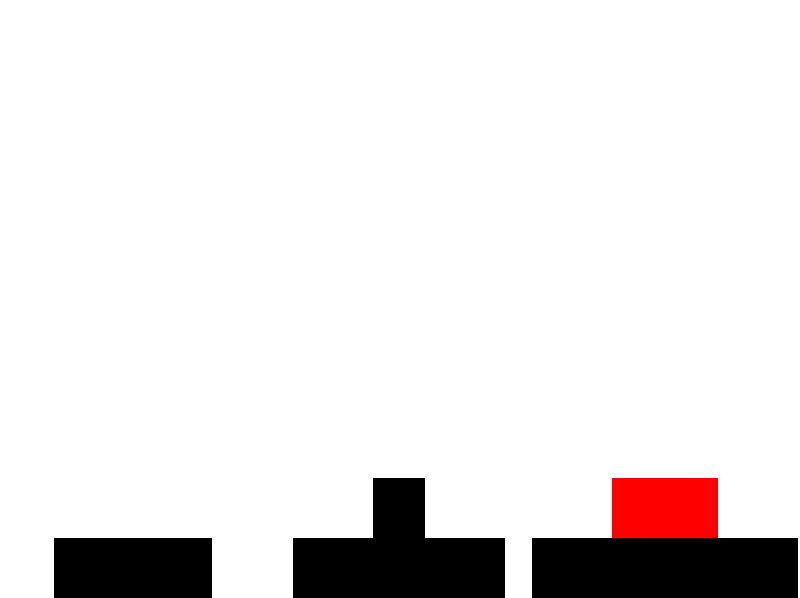
\includegraphics[scale=0.2]{../diapo/anim_hanoi.png}
\end{center}
\label{fig:hanoiimg}
\end{figure}

\clearpage
\section{Annexe - Penrose}
\begin{algorithm}[H]
\label{algo:penrose}
  \SetKwInOut{Input}{Entrées}
  \caption{Penrose($n$, $t$)}
  \label{alg:penrose}
  \Input{$n$ : nombre de générations, \newline
  $t$ : triangle initial}
  \eIf{$n = 0$}{ dessiner $t$}
  { Découper $t$ et appliquer Penrose($n-1$,$t_i$) pour chaque sous triangle $t_i$.
   }
\end{algorithm}

\begin{figure}[h]
  \begin{center}
    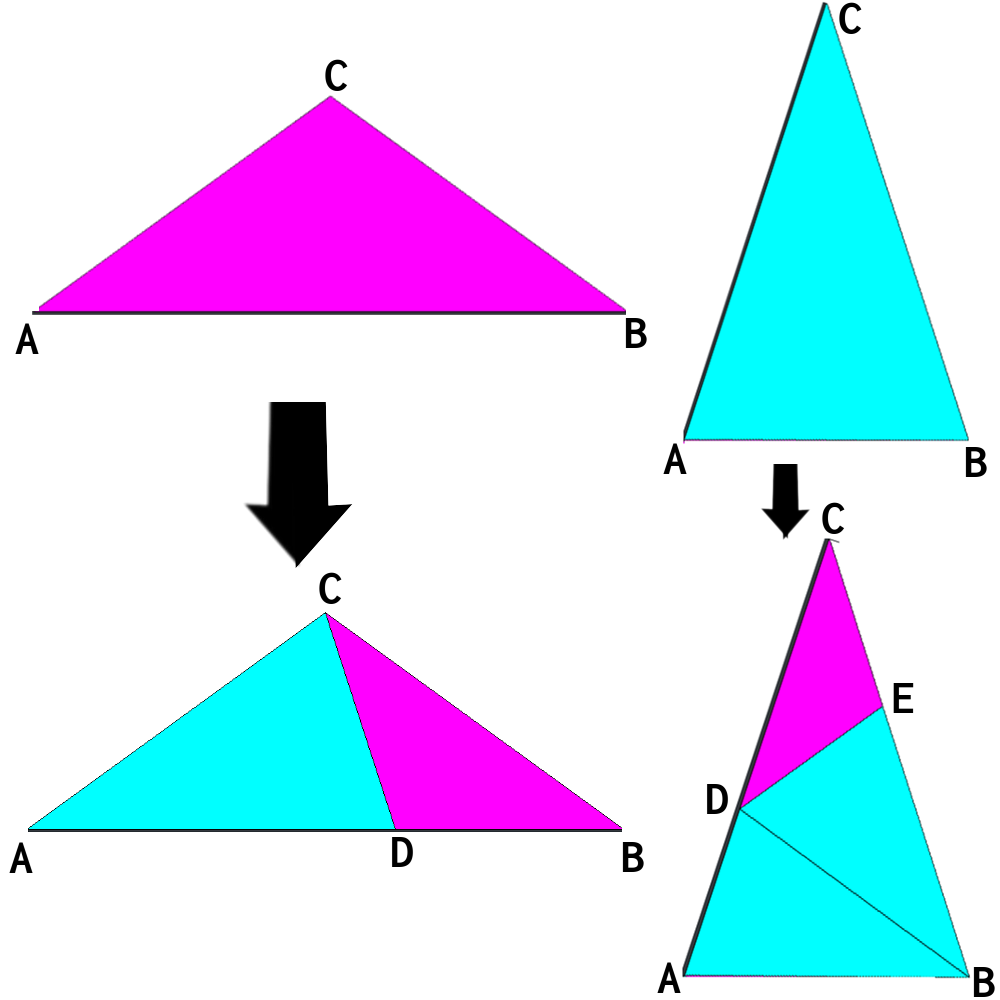
\includegraphics[width=12cm]{triangle-generation1.png}
    \caption{Division des triangles (obtus à gauche, aïgus à droite.}
    \label{fig:decoupage1}
  \end{center}
\end{figure}


\begin{figure}[h]
\begin{center}
\begin{tikzpicture}[node distance=1.5cm,
    every node/.style={fill=white, font=\sffamily}, align=center]
  % Specification of nodes (position, etc.)
  \node (penrosebase) at (0,0)           [mainFile]          {penrose\_base.ml};
  \node (trgraphics) at (-3,-2)     [subFile]        {trgraphics.ml};
  \node (apitriangle) at (3, -2)     [module] {api\_triangle.cma};
  % Specification of lines between nodes specified above
  % with aditional nodes for description
  \draw[->]             (penrosebase) -- (apitriangle);
  \draw[->]     (penrosebase) -- (trgraphics);
  \draw[->]      (trgraphics) -- (apitriangle);
\end{tikzpicture}
\caption{Relations entre les fichiers}.
\label{fig:filesrelation}
\end{center}
\end{figure}

\begin{figure}[h]
\inputminted[frame=lines,linenos]{ocaml}{../penrose/api_triangle.mli}
\caption{api\_triangle.mli}
    \label{code:apitrianglemli}
\end{figure}

\end{document}
